\documentclass[12pt]{article}
	
%______________________PREAMBULO_________________________

%----------------------Paquetes--------------------------
\usepackage{amsmath,amssymb,amsfonts,latexsym,cancel} % Paquetes de símbolos adicionales.
\usepackage[spanish,es-tabla]{babel} % Idioma español
\usepackage[utf8]{inputenc} % Paquete que nos permite usar los acentos y otros símbolos, directamente del teclado.
\usepackage[T1]{fontenc} % Cambia el tipo de letra
\usepackage{times} % Tipo de letra Times New Roman
\usepackage{graphicx} % Paquete para el manejo de gráficos y figuras en el documento.
\usepackage{geometry} % Permite el manejo de los margenes
\usepackage{fancyhdr} % Permite colocar y manejar el encabezado
\usepackage[breaklinks,colorlinks=true,linkcolor=black,citecolor=blue, urlcolor=blue]{hyperref} % Crea hipervinculo entre secciones y el indice
\usepackage{pstricks}
\usepackage{multicol}
%\usepackage{mathpazo} %fuente palatino
%\usepackage{xcolor}
%\usepackage[shortlabels]{enumitem}
%-------------Paquetes para el formato de las citas-------
%\usepackage[hyphens]{url}
%\usepackage{float}
%\usepackage{cite}
%\usepackage{wrapfig}

%-----------------------------ayuda de paquetes--------------------

\spanishdecimal{.}

%------------------------Margenes----------------------------

\newgeometry{bottom = 2.5 cm, top = 2.5 cm, left = 2 cm, right = 2 cm} % Modifica el margen {Abajo, Arriba, Izquierda, Derecha

%----------------------------Interlineado----------------------------------

%\doublespacing
%\onehalfspace
%\singlespace
%\spacing{1.5} % Permite personalisar a gusto
%\setlength{\parskip}{2cm} % Es el espacio entre parrafos

%-----------------------------Sangria---------------------------------------

\setlength{\parindent}{0 cm} % Manipula la sangria

%---------------------Portada------------------

%\title{
%\begin{figure}[h!]
		
%	\centering
%	
\includegraphics[width=\linewidth]{Nom_UAdeC_FCFM.png}  			
			
%\end{figure}
%\huge \textbf{LABORATORIO DE FISICA 3}\\\LARGE TITULO PRACTICA\\}
%\author{ \Large \textbf{Profesor:}\\
%\Large \textbf{Alumno:} Oscar Joel Castro Contreras}
%\date{\today}

%--------------Encabezado y pie de pagina--------------------

\pagestyle{fancy}%Coloca el encabezado en el documento
\lhead[]{Métodos numéricos}%Encabezado izquierda
\rhead[]{Oscar Joel Castro Contreras}%Encabesado derecha
%\chead[]{}%Encabesado central
\renewcommand{\headrulewidth}{0.08 pt}%Coloca linea al pie de pagina

%\lfoot[]{PI}%Pie de pagina izquerdo
%\rfoot[]{PD}%Pie de pagina derecho
\cfoot[]{\thepage}%Pie de pagina central
\renewcommand{\footrulewidth}{0.08 pt}%Coloca linea al pie de pagina

%-----------------------------------------------------------------------------

	\begin{document}
		
		\begin{titlepage}
		
			\centering
			{\bfseries
			\begin{figure}[h!]
				\centering
				
\includegraphics[width=\linewidth]{Nom_UAdeC_FCFM.png} 				
			\end{figure}
			\par}
			\vspace{2cm}
			{\scshape\LARGE Métodos Matematicos \par}
			\vspace{3cm}
			{\scshape\Huge \textbf{Método de Horner} \par}
			\vfill
			{\LARGE \textbf{Profesora:} Maria Guadalupe Godina Cubillo \par}
			\vspace{3cm}
			{\LARGE \textbf{Alumno:} Oscar Joel Castro Contreras \par}
			\vfill
			{\Large \today \par}
			\thispagestyle{empty}
			%\thispagestyle{fancy}
			
		\end{titlepage}
	
		\newpage

		\begin{abstract}
			\noindent En este reporte explico un poco de los métodos que existen para encontrar las raíces de cualquier 
			polinomio o función que tenga raíces, y en específico explico, qué es, en que consiste y cuales son las 
			limitaciones del método de Horner para encontrar raíces de polinomios.
		\end{abstract}

		\textbf{Palabras clave:} Raíces, Horner, División sintética, Maximo, Mínimo.

		\section*{\centering Introducción}\label{sec:Introducción}
			Los polinomios son uno de los conceptos más importantes en álgebra y son fundamentales en 
			matemáticas y ciencia en general. Determinar las raíces de un polinomio es uno de los problemas 
			más antiguos en matemáticas.\\
			Puesto que las ecuaciones polinomiales aparecen en un amplio rango de áreas de la ciencia, desde 
			química y física básica hasta economía, el problema de determinar raíces de polinomios es, con 
			frecuencia, un paso obligado en la resolución de problemas.\cite{bib:item1}\\
			La razón principal para resolver ecuaciones no lineales por medio de métodos computacionales es 
			que algunas ecuaciones carecen de solución exacta, excepto por unas pocas. Por lo que existen 
			métodos numéricos diseñados para obtener las raíces, aunque cada uno tiene sus propias 
			limitaciones y defectos. Algunos métodos se muestran en la tabla \ref{tab:1}.\cite{bib:item2}\\
			\begin{table}[h!]
				\centering
				\begin{tabular}{|c|c|}
					\hline
					\multicolumn{2}{|c|}{\textbf{Métodos numéricos para obtener raíces}}\\
					\hline
					\textbf{Nombre} & \textbf{Características} \\\hline
					Bisección & Aplicable a funciones no analiticas \\\hline
					Regla falsa & Convergencia lenta en un intervalo grande \\\hline								
					Método de Newton & Rápido, se nesecita calcular derivada \\\hline
					Método de secante & Rápido, no se requiera calcular derivada \\\hline
					Sustitución sucesiva & Puede no converger \\\hline
				\end{tabular}
				\caption{Métodos numéricos para obtener raíces \cite{bib:item2}}
				\label{tab:1}
			\end{table}\\
			En general, no es posible determinar los ceros de una función, es decir, valores $ x^* $ tal que $f(x^*) = 0 $, 
			en un número finito de pasos. Tenemos que usar métodos de aproximación. Los métodos son 
			usualmente iterativos y tienen la forma: Iniciando con una aproximación inicial $ x_0 $ (o un intervalo $ [a,b] $) , 
			se calculan aproximaciones sucesivas $ x_1,x_2,... $ y elegimos $ x_n $ como aproximación de $ x^* $ cuando se cumpla un 
			criterio de parada dado. A los ceros de un polinomio se les conoce también como raíces.\\
			\textbf{El método de Horner:}\\
			Llamado así en honor del maestro de escuela británico William George Horner quien lo describió 
			en 1819. Se trata de un método que es utilizado para aproximar una raíz real de una ecuación 
			polinómica.\cite{bib:item3} \\
			Al usar el método de Newton para localizar los ceros aproximados de un polinomio $ P(x) $, 
			necesitamos evaluar $ P(x) $ y $ P'(x) $ en valores específicos. Puesto que tanto $ P(x) $ 
			como $ P'(x) $ realice de la manera anidada. El método de Horner incorpora esta técnica 
			anidada y como consecuencia, sólo requiere n multiplicaciones y n sumas para evaluar un 
			polinomio de enésimo grado.\cite{bib:item4} \\
			Sea $$ P(x) = a_nx^n + a_{n-1}x^{n-1} + \cdots + a_1x + a_0 $$ 
			Defina $ b_n = a_n $ y $$ b_k = a_k +b_{k+1}x_0, \quad k = n-1, n-2,\ldots, 1, 0. $$
			Entonces $ b_0 = P(x_0) $. Además, si $$ Q(x) = b_nx^{n-1} + b_{n-1}x^{n-2} +\cdots+ b_2x + b_1, $$ 
			Entonces $$ P(x) = (x-x_0)Q(x) + b_0. $$
			Por definición de $ Q(x) $
			\begin{align*}
				(x-x_0)Q(x) + b_0 &= (x-x_0)(b_nx^{n-1} + b_{n-1}x^{n-2} +\cdots+ b_2x + b_1) + b_0 \\
				&= (b_nx^{n} + b_{n-1}x^{n-1} +\cdots+ b_2x^2 + b_1x) \\
				&= (b_nx_0x^{n-1} +\cdots+ b_2x_0x^2 + b_1x_0) + b_0 \\
				&= b_nx^n + (b_{n-1} - b_nx_0)x^{n-1} +\cdots+ (b_1 + b_2x_0)x + (b_0 -b_1x_0).
			\end{align*}
			Por la hipótesis, $ b_n = a_n $ y $ b_k - b_{b+1}x_0 = a_k $, por lo que
			$$ (x-x_0)Q(x) + b_0 = P(x)\text{ y }b_0 = P(x_0) $$

		\section*{\centering Metodología}\label{sec:Metodologia}
			El método de Horner para encontrar raíces solo puede ser usado para polinomios, el método 
			consiste en tomar un polinomio $P(x) $, y dar un punto $ x_0 $ que este cercano un de sus 
			raíces reales, con la ayuda de este punto y de la división sintética se reducirá el polinomio 
			a uno de grado menor $ Q(x) $, de esta división sintética guardamos lo que vale la evaluación 
			de $ P(x_0) $.
			\begin{table}[h!]
				\centering
				$ P(x) = a_4x^4 + a_3x^3 + a_2x^2 + a_1x + a_0,\quad x_0 $ \\
				\begin{tabular}{ccccc|c}\\
					$a_4$ & $a_3$ & $a_2$ & $a_1$ & $a_0$ & \\
					 & $b_4x_0$ & $b_3x_0$ & $b_2x_0$ & $b_1x_0$ & $x_0$ \\\hline							
					$b_4$ & $b_3$ & $b_2$ & $b_1$ & $b_0$ & $ P(x_0) = b_0$ \\
				\end{tabular}
			\end{table}\\
			Después, volvemos a realizar división sintética con el mismo punto $ x_0 $ y el polinomio que 
			reducido $ Q(x) $ y de esta división sintética guardamos lo que vale $ Q(x_0) $.\\
			\begin{table}[h!]
				\centering
				$ Q(x) = b_4x^3 + b_3x^2 + b_2x + b_1 $ \\
				\begin{tabular}{cccc|c}\\
					$b_4$ & $b_3$ & $b_2$ & $b_1$ & \\
					 & $c_4x_0$ & $c_3x_0$ & $c_2x_0$ & $x_0$ \\\hline							
					$c_4$ & $c_3$ & $c_2$ & $c_1$ & $ Q(x_0) = c_1$ \\
				\end{tabular}
			\end{table}\\
			Al final usamos la formula del método de Newton Raphson para obtener una aproximación, y tomamos 
			a $ Q(x_0) $ como si fuera la derivada. Después, tomamos la aproximación obtenida e iteramos 
			realizando todo el procedimiento de nuevo.
			$$ x_1 = x_0 - \frac{P(x_0)}{Q(x_0)} $$
			\begin{center}
				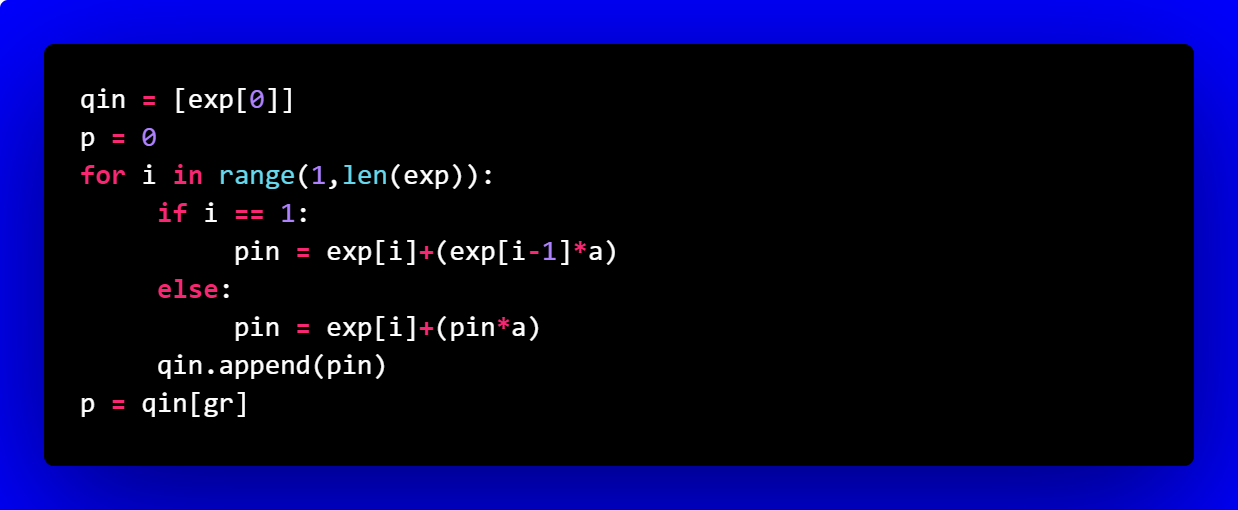
\includegraphics[width=\linewidth]{Figura 1.png}
				Figura 1: La división sintética de un polinomio en codigo			
			\end{center}
			Esta parte de mi programa realiza las divisiones sintéticas, tomando los coeficientes del polinomio 
			y retornando el valor de $ P(x_0) $ o $ Q(x_0) $.
		
		\section*{\centering Resultado}\label{sec:Resultado}
			Si tomamos el polinomio $ x^3-2x^2-1 $ y damos el punto $ x = 1 $. Hacemos 
			la evaluación para obtener la raíz con 5 cifras significativas, el programa nos arroja
			\begin{multicols}{2}
				\begin{center}
					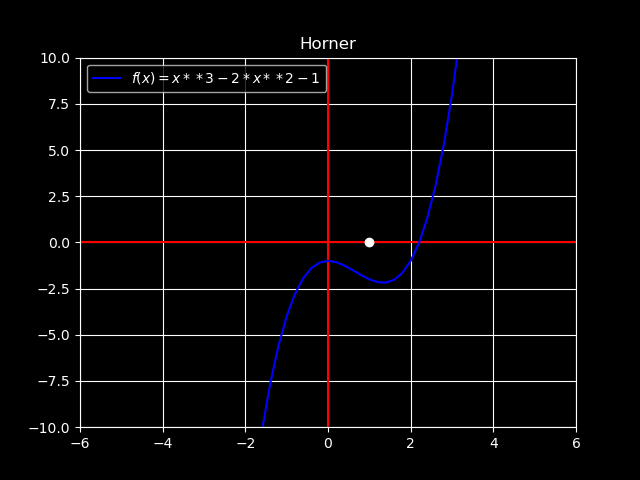
\includegraphics[width=\linewidth]{Grafica 1.png}
					Grafica 1: Punto aproximado a la raíz dado \columnbreak $ x^3-2x^2-1 $ en $ x = 1 $.\\
					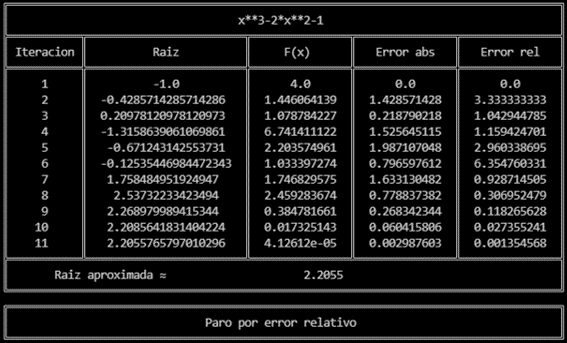
\includegraphics[width=\linewidth]{Tabla 1.png}
					Tabla 2: Iteraciones a la aproximación de la raíz de la función $ x^3-2x^2-1 $.
				\end{center}
			\end{multicols}
			Observamos que la aproximación a la raíz es $ 2.2055 $, con 11 iteraciones. El criterio de paro fue 
			por el error relativo. \\

		\section*{\centering Observación}\label{sec:Observacion}
			El método tiene una limitación, la cual ocurre cuando $ Q(x_0) = 0 $, cuando ocurre esto es por 
			que el punto donde se da la aproximación es un máximo o un mínimo de la función, en estos casos 
			el método se detiene y se tiene que iniciar de nuevo pero dando otra aproximación que no sea un 
			mínimo o un máximo.

		\section*{\centering Conclusión}\label{sec:Conclusion}
			En conclusión, el método de Horner solo puede encontrar raíces reales de polinomios, tomando 
			una aproximación inicial $ x_0 $ y con la ayuda de la división sintética y la aproximación, 
			obtener $ P(x_0) $ y $ Q(x_0) $ los cuales se sustituyen en la formula del método de Newton Raphson, 
			tomando a $Q(x_0) $ como la derivada. \\
			Sus limitaciones es cuando la aproximación cae en un máximo o un mínimo de la función en estos casos 
			$ Q(x_0) = 0 $, por lo que el método se detiene.

		\centering
		\begin{thebibliography}{10}
			\bibitem{bib:item1} de la Vega, H. M. El calculo de raıces de polinomios. Una historia sin fin. Recuperado de
							\href{http://www.matedu.cinvestav.mx/~elcalculoysuensenanza/investigacion/articulosPDF/Madrid.pdf}{Pagina web de \cite{bib:item1}}.
			\bibitem{bib:item2} Nakamura, S. (1998). Metodos Numericos Aplicados Con Software. En Solución de ecuaciones no lineales (Primera ed., pp. 62–63). Prentice Hall.
			\bibitem{bib:item3} Restrepo García, C. J. (2019). Un estudio histórico sobre la aproximación a las raíces reales de una ecuación polinómica a través del método 
							de Horner como recurso para la enseñanza de ecuaciones en grado 10° de la Educación Media.
							\href{https://bibliotecadigital.univalle.edu.co/bitstream/handle/10893/21225/CB%200525927-3487.pdf?sequence=1&isAllowed=y}{Pagina web de \cite{bib:item3}}.
			\bibitem{bib:item4}	Burden, A. M., Faires, D. J. (2017). Análisis numérico (10a. ed.). En Método de Horner (10a. ed., pp. 69–72). Cengage Learning.
		\end{thebibliography}

	\end{document}